\documentclass[a4paper,10pt]{article}
\usepackage[utf8]{inputenc}
\usepackage[french]{babel}
\usepackage{amsmath}
\usepackage[osf,sups]{Baskervaldx} % lining figures
\usepackage[bigdelims,cmintegrals,vvarbb,baskervaldx]{newtxmath} % math font
\usepackage{graphicx}
%\usepackage{url,hyperref}

% margins
\setlength{\parindent}{0em}
\setlength{\parskip}{1em}
\addtolength{\hoffset}{-4.5em}
\addtolength{\textwidth}{11em}
\addtolength{\voffset}{-5em}
\addtolength{\textheight}{10em}

\begin{document}
\thispagestyle{empty}

{\bf
	%Calcul numérique des fonctions de Mathieu et de leurs racines.
	Fonctions de Mathieu: modélisation, analyse et simulation.
}

{\bf Encadrants}:\\
Enric Meinhardt-Llopis \verb+<enric.meinhardt@ens-paris-saclay.fr>+\\
Rafael Grompone von~Gioi \verb+<rafael.grompone@ens-paris-saclay.fr>+

{\bf Contexte.}
Les fonctions propres du Laplacien dans un domaine elliptique
\vspace{-1em}
\begin{center}
	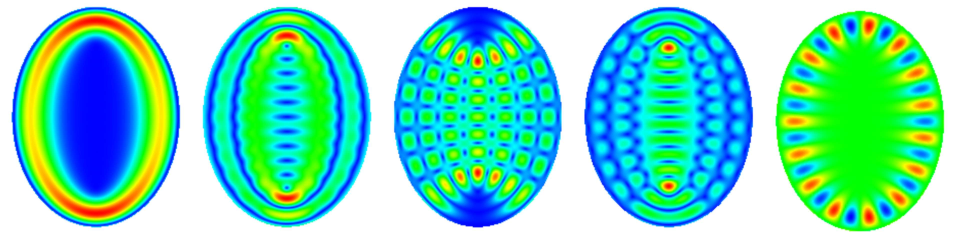
\includegraphics[width=0.9\linewidth]{f/ellnice.png}
\end{center}
\vspace{-2em}
ont beaucoup d'applications en science et technologie. Plus important:
l'ellipse est une des seules six formes dont on sait calculer
explicitement %~\cite{localfun,geofun}
les fonctions propres (avec le rectangle, le disque, le triangle équilatéral,
le demi-triangle équilatéral~30-60-90 et le le triangle isocèle rectangle).  En
coordonnées elliptiques, ces fonctions propres sont à variables
séparées~$\varphi_{i,j}(\rho,\theta)=M_i(\rho)S_j(\theta)$ où~$\{M_i\}$
et~$\{S_j\}$ sont deux familles dénombrables de fonctions, dites
les~\emph{fonctions de Mathieu} radiales et périodiques
respectivement.  %~\cite{abramo}.
Les fonctions de Mathieu sont les solutions des
équations différentielles ordinaires suivantes:
\[
	y''-(a-2q\cosh(2x))y = 0
	\qquad
	\qquad
	y''+(a-2q\cos(2x))y = 0
\]
lesquelles sont très bien conditionnées et on sait résoudre par des méthodes
classiques.

%SCRIPT plambda zero:1x10000 ":j :h / 7 * dup  7 46 rox3 mathieu-ce join" -o TXT:-|gnuplot -e 'set term pngcairo crop size 500,300;unset key;plot [0:2*pi] [-1.5:1.5]  0,"-" w lines' > f/mathieu_periodic.png
%SCRIPT plambda zero:1x10000 ":j :h / 7 * dup  5 1 rox3 mathieu-Ms1 join" -o TXT:-|gnuplot -e 'set term pngcairo crop size 500,300;unset key;plot [0:6] [-0.5:0.5]  0,"-" w lines' > f/mathieu_radial.png

\vspace{-1em}
\begin{center}
\begin{tabular}{cc}
	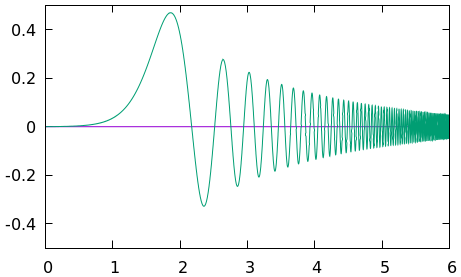
\includegraphics[width=0.3\linewidth]{f/mathieu_radial.png} &
	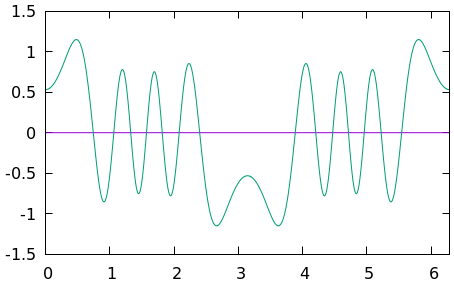
\includegraphics[width=0.3\linewidth]{f/mathieu_periodic.png} \\
	Mathieu radiale~$M_5(\rho)$ & Mathieu périodique~$S_{46}(\theta)$
\end{tabular}
\end{center}
\vspace{-1em}
Pour construire les fonctions propres~$\varphi_{i,j}$ à la bonne échelle, il
faut calculer les fonctions de Mathieu, et également toutes
leurs racines, ainsi que les racines de leurs dérivées premières.

Malheureusement, aucun des logiciels mathématiques librement disponibles (GNU
Scientific Library, SciPy, Octave, etc.) ne propose pas un calcul des racines
de Mathieu.  Le calcul explicite des fonctions propres de l'ellipse n'est donc
pas possible en pratique!

{\bf Objectif du stage.}
L'objectif initial du stage est d'écrire un algorithme pour le calcul des
racines des fonctions de Mathieu.  À cet objet, on étudiera d'abord la théorie
(élémentaire) des fonctions de Mathieu et l'algorithme classique pour les
évaluer.  La méthode proposée pour évaluer les racines consiste d'abord à faire
une approximation initiale (par exemple les racines de~$M_n(\rho)$ sont très
proches de celles de~$\sin(\exp(n\rho))$ comme on voit dans la figure), et
ensuite quelques itérations de la méthode de Newton.

Si le stage amène à une conclusion positive, on proposera l'inclusion du calcul
de racines aux auteurs des principaux logiciels libres, afin de permettre à
tout le monde de calculer les modes de vibration d'une ellipse.  Comme
application, on pourra aussi essayer de simuler le phénomène
des~\emph{cicatrices quantiques} (quantum scarring).  Ces
cicatrices sont des statistiques de grandes familles de fonctions propres qui
laissent voir la forme de certaines trajectoires périodiques.  Jusqu'à
l'instant, celles-ci n'ont jamais été observées dans un domaine elliptique,
probablement dû à la manque de support informatique pour les fonctions de
Mathieu.



\vspace{-1.5em}
\renewcommand{\refname}{\normalsize Références}
%
\begin{thebibliography}{99}
\vspace{-1em}
{\scriptsize
%\bibitem{drum}
%	Kac, M..
%	{\it Can one hear the shape of a drum?}
%	The american mathematical monthly, (1966)
%
%\bibitem{inverse}
%	Chu, M., \& Golub, G.
%	{\it Inverse eigenvalue problems: theory, algorithms, and
%	applications}, OUP (2005)
%
\bibitem{localfun}
	Nguyen, B. \& Grebenkov, D.~S.
	{\it Localization of Laplacian eigenfunctions in circular, spherical
	and elliptical domains}, SIAM J.  Appl. Math. (2019)

\bibitem{geofun}
	Grebenkov, D.~S.  \& Nguyen, B.
	{\it Geometrical structure of Laplacian eigenfunctions},
	SIAM Rev. (2013)

\bibitem{abramo} Abramowitz, M. \& Stegun, I.
	{\it Handbook of mathematical functions, with
	formulas, graphs, and mathematical tables.} (1965)

\bibitem{dietz}
	Dietz, B.
	{\it Circular and Elliptical Neutrino Billiards:
	A Semiclassical Approach.}
	Proc. Workshop on Quantum Chaos and Localizaton Phenomena (2019)

%
%\bibitem{backeigen}
%	Wang,~W., Dang,~Z., Hu,~Y., Fua,~P., Salzmann,~M.
%	{\it Backpropagation-Friendly Eigendecomposition},
%	NeurIPS (2019)
%
}
\end{thebibliography}



\end{document}  


% vim:set tw=79 spell spelllang=fr:
